%% PHYSICS:
\documentclass[submission, Phys]{SciPost}

% Prevent all line breaks in inline equations.
\binoppenalty=10000
\relpenalty=10000

\hypersetup{
    colorlinks,
    linkcolor={red!50!black},
    citecolor={blue!50!black},
    urlcolor={blue!80!black}
}

\usepackage[bitstream-charter]{mathdesign}
\urlstyle{sf}
\usepackage{subcaption}
\usepackage{float}

% Fix \cal and \mathcal characters look (so it's not the same as \mathscr)
\DeclareSymbolFont{usualmathcal}{OMS}{cmsy}{m}{n}
\DeclareSymbolFontAlphabet{\mathcal}{usualmathcal}

\usepackage[varvw]{newtxmath}

\begin{document}

% The article title is centered, Large boldface, and should fit in two lines
\begin{center}{\Large \textbf{
Domain Wall Dynamics for a 1D Bose gas\\
}}\end{center}

% TODO: write the author list here. Use first name (+ other initials) + surname format.
% Separate subsequent authors by a comma, omit comma and use "and" for the last author.
% Mark the corresponding author with a superscript star.
\begin{center}
Léa Dubois\textsuperscript{1}, G. Themèze, J. Dubail and I. Bouchoule,
% Aah B. Cee\textsuperscript{1} and
% Gee K. See\textsuperscript{2$\star$}
\end{center}

% TODO: write all affiliations here.
% Format: institute, city, country
\begin{center}
{\bf 1} Laboratoire Charles Fabry, Institut d'Optique, Université Paris-Saclay
% \\
% {\bf 2} Affiliation2
% \\
% {\bf 3} Affiliation2
\\
% TODO: provide email address of corresponding author
${}^\star$ {\small \sf lea.dubois@universite-paris-saclay.fr}
\end{center}

\begin{center}
\today
\end{center}

% For convenience during refereeing (optional),
% you can turn on line numbers by uncommenting the next line:
%\linenumbers
% You should run LaTeX twice in order for the line numbers to appear.

\section*{Abstract}
{\bf
Abstract
}


% Guideline: if your paper is longer that 6 pages, include a TOC
% To remove the TOC, simply cut the following block
\vspace{10pt}
\noindent\rule{\textwidth}{1pt}
\tableofcontents\thispagestyle{fancy}
\noindent\rule{\textwidth}{1pt}
\vspace{10pt}

List of figures  : 
\begin{itemize}
    \item For the experimental setup : atom chip with the shape of the longituinal trap + linear density profil of the initial situation
    \item For the experimental data : Euler scale observed
    \item For the experimental data : edge profile with (T=0, Lieb-Liniger) and (T=0, GP) 
    \item experimental edge profile + fit by GE + fit of the left part by GE + fit of the right part by GE + insert avec fig. 9.9 de la thèse de Léa \textbf{enlever les ajustements thermiques gauches et droites}
    \item (a) experimental edge profile + fit by  function s (4 fittng parameters) ; (b) distribution des facteurs d'occupation (c) distributions de rapidités
    %\item Non thermal ansatz : Thermal and non thermal occupation factor (and rapidity distribution ???) + superposition with the experimental profile.
    \item  local rapdity distribution : voir dernière figure déjà mise 
\end{itemize}

\section{Introduction} 
%[Permier jet : Isabelle]
\label{sec:intro}

Gaining insight on the out-of-equilibrium dynamics of many-body quantum systems is tremendously difficult and it is the goal of an active research field.  
One particular class of systems where important progress have been done is the class of integrable one-dimensional systems. 
%In contrast to ergodic systems 
%which relaxe, as long as local observable are concerned, towards thermal states parametrized by a few quantities, the quilibrium states which emerge after relaxtion in intergable systems are parametrised by a whole function, their rapidity distribution[]. 
Owing to their infinite number of local conserved charges, to describe the local properties of equilibrium states that arise after relaxation, one needs a  whole function, the rapidity distribution[]. 
The latter can be viewed as the distribution in velocity space 
of the infinite-lifetime quasi-particles in the system. Large scale dynamics is 
accounted for by a generalized hydrodynamic (GHD) effective theory[], which 
assume local equilibrium.
A paradigmatic situation that can be handled by  this theory is the dynamics 
induced by a partite quench\cite{bertini_transport_2016,castro-alvaredo_emergent_2016}, dubbed  domain-wall protocol in this paper. In this protocol the Hamiltonian governing the  dynamic is translation invariant but the initial state is the junction of two semi-infinite 
homogeneous systems each prepared in a different equilibrium state from the Hamiltonian. The GHD theory predicts that, at time long enough such that diffusion effects become negligible\cite{de_nardis_diffusion_2019} and Euler-scale hydrodynamics is valid,  the time evolution is ballistic. % and the local state a time $t$ after the junction and at a position $x$ from the merging point is solely a function of $x/t$. 
An interesting feature of this protocol is that the local state, within the merging region, is expected to present features
characteristic of zero-temperature systems. Thus, this protocol could be used to reveal power-law singularities of correlation function characteristic of zero-temperature Luttinger liquid\cite{de_nardis_edge_2018}, providing a local  probe is performed. 

In this paper, we experimentally realize an instance of the domain-wall protocol
using an ultra-cold atomic Bose gas, well described by the Lieb-Liniger model of 
one-dimensional Bosons with contact repulsive interactions\cite{lieb_exact_1963,bouchoule_generalized_2022}, which is an integrable model. 
The domain wall consists in our experiment in the junction of a gas prepared in an equilibrium state on the one side, and the vacuum on this other side. It is prepared, starting from a homogeneous cloud, by the sudden removal of its left part. For different evolution times, we record the density profile of the border between the two zones, dubbed the border profile. We find that the border profile shows a ballistic behavior, as expected from GHD theory at Euler scale. 

The border profile, for clouds prepared with deep evaporative cooling, is in fair agreement with GHD predictions assuming the semi-infinite gas is in its ground state, although deviations are present. We show that, from the border profile, it is in principle possible to reconstruct the rapidity distribution characterizing the initial gas. This protocol can thus be used as a generalized thermometry. 
However, the reconstruction method suffers from a high sensitivity to experimental noise in the tail of the border profile, which prevent us to reconstruct faithfully the initial rapidity distribution. Instead, we use an ansatz parametrized by a few parameters to extract the rapidity distributions of the initial gas from a fit to the border profile. 

Finally, we use a newly developed techniques\cite{dubois_probing_2024} to probe the local rapidity distribution within the border. The latter is expected to be highly asymmetric for an initial state whose rapidity distribution is substantially broader and 
smoother than that of the ground state:  while one of its border 
reflects the broad character of the initial rapidity distribution, the other border 
present the sharp feature expected for the ground state.  Our experimental data show such an asymmetric behavior, although the above feature is softened by the finite spatial resolution of the local rapidity distribution measurement.  


%\begin{itemize}
%    \item Introducing GHD to introduce the protocol : introducing the problem in terms of rapidity distribution and in terms of occupation factor.
%\end{itemize}


\section{Experimental setup}
%\subsection{Atom chip experiment}

We produce an ultra-cold gas of $^{87}$Rb bosonic atoms in the stretched state $|F=2,m_F=2 \rangle$ using an atom chip. In addition to a homogeneous longitudinal magnetic field $B_0 = 3.36 $G, transverse trapping is achieved with three parallel microwires deposited on the chip (shown in blue in Fig.\ref{fig:setup}(a)) which carry AC currents at $400$MHz. This configuration eliminates wire roughness effects and allows independent control over both longitudinal and transverse confinement \cite{PhysRevLett.98.263201}. The atoms are trapped $7\mu$m from the chip surface and $15\mu$m from the wires, enabling strong transverse confinement. The transverse trapping potential used in the following is harmonic, with a frequency of $\omega_{\perp}/ 2 \pi=2.56 $kHz. 
Using radio-frequency evaporative cooling, we produce an atomic cloud at a temperature of approximately $T=100$nK and a chemical potential of $\mu/ k_B = 45$nK. With these parameters, $\mu/ (\hbar \omega_{\perp})=0.4$ and $k_B T/ (\hbar \omega_{\perp} )=0.8$, the gas enters in the $1$D regime. The effective 1D coupling constant for atoms in the transverse ground state is given by $g = 2 a_{3D} \hbar \omega_{\perp}$ where $a_{3D}$ is the $3$D scattering length of $^{87}$Rb \cite{PhysRevLett.81.938}. Further details on the setup can be found in \textbf{REF}. 

% To experimentally study domain wall dynamics in $1$D Bose gases, it is essential to achieve a quasi-homogeneous atomic density over a relatively large region. To this end, we decided to use a longitudinal quartic magnetic trap produced by DC currents through four wires positioned on either side of the three microwires, as shown in the Fig.\ref{fig:setup}(a). Since these wires are placed far from the center of the chip, the longitudinal potential can be expressed as a polynomial series expansion $V(x)= \sum_{i} a_i x^i$. 

The longitudinal magnetic trap is produced by DC currents through four wires positioned on either side of the three microwires, as shown in the Fig.\ref{fig:setup}(a). Since these wires are placed far from the center of the chip, the longitudinal potential can be expressed as a polynomial series expansion $V(x)= \sum_{i} a_i x^i$. 
The fourth first coefficients $a_i$ are tuned by adjusting the currents in the four wires that generate the longitudinal trapping potential. By carefully selecting these currents, it is possible to set $a_1$, $a_2$ and $a_3$ to zero. Since the higher-order coefficients $\{a_i\}_{i>4}$ can be neglected, setting $a_1$, $a_2$, and $a_3$ to zero produces as a first appxoimation a quartic potential. This potential shape is particularly useful in our case: to experimentally study domain wall dynamics in 1D Bose gases, it is important to achieve a quasi-homogeneous atomic density over a relatively large region. The quartic potential satisfies these requirements.
An example of linear density extracted from an atomic cloud placed in such a potential is represented in gray in Fig.\ref{fig:setup}(b). The linear density $n_0$ remains constant to within $10 \%$ around the peak density over a range of approximately $250 \mu$m. 

% We can restrict ourselves to the first $4$ predominant terms giving $V(x) = \sum_{i=1}^{4} a_i x^i$. The coefficients $a_i$ are tuned by adjusting the currents in the four wires. By carefully selecting these currents, it is possible to set $a_1$, $a_2$ and $a_3$ to zero, resulting in a quartic potential, the superior coefficients being negligible.

With a near-zero dimensionless Lieb parameter $\gamma =  mg / (\hbar^2 n_0) \in [0.4,0.7] \times 10^{-2}$ and a temperature $ T \ll n_0^{3/2} \sqrt{\hbar^2 g /m}/k_B$, the atomic clouds produced are deeply in the quasicondensate regime, where density fluctuations are almost completely suppressed, but phase fluctuations remain \cite{PhysRevLett.91.040403}.

%\subsection{Producing an initially semi-infinite homogeneous 1D Bose gas}\label{sub_pisih}

To produce an initially semi-infinite homogeneous gas, we use the selection method introduced in \cite{PhysRevLett.133.113402}. We illuminate an edge of the atomic cloud, initially in equilibrium in a quartic trap, with light that is nearly resonant with the $F=2 \to F' = 3$ transition of the $D2$ line. Atoms shined by this light are subjected to radiation pressure : after being illuminated for $30 \mu$s corresponding to $\sim 15$ absorption/reemission cycles, they are no longer trapped. To illuminate only an edge of the gas, the beam is shaped using a digital micromirror device (DMD). Further details on this spatial selection method are available in \cite{PhysRevLett.133.113402}. This protocol produces a clean edge between a zero density system and a homogeneous gas due to the fact that the atoms are initially placed in a quartic trap. An example of the density profile of a gas initially in equilibrium in a quartic trap, after applying this spatial selection tool, is shown in yellow in Fig.\ref{fig:setup}(b). The gas is then homogeneous to within $10 \%$ over a distance of approximately $200 \mu$m. 

The longitudinal confinement is then removed while maintaining the transverse confinement. The initial sharp border braodends in time 
and this  dynamics is monitored by recording longitudinal density profiles $n(x,t)$ after different evolution time $t$. %to investigate the longitudinal dynamics.
\begin{figure}[!htb]
    \centering
    \includegraphics[width=1.0\linewidth]{Figures/Atom_chip.PNG}
    \caption{(a) Schematic drawing of the atom chip. The $3$ blue wires produce the transverse trapping, the $4$ other wires produce the longitudinal trapping. The red oval ball represents the atomic cloud, trapped 15 microns above the wires $-$ (b) The gray curve represents the linear density profile of gas confined within a quartic potential. The atomic cloud is then illuminated during $30 \mu$s by a near resonant light beam, shaped using a DMD. The resulting density profile is depicted in yellow.}
    \label{fig:setup}
\end{figure}

\section{GHD predictions}\label{sec.GHDpredictions}
%{\bf [Premier jet : Isabelle]}
Under time evolution, the initial sharp border of the cloud smoothens, and the time
derivative of local quantities decrease. 
After some time, %Once its extension is large compared to microscopic length scales, 
upon coarse graining in position and time, one expects that the gas can locally be described by equilibrium states.
%is locally in equican 
%describe the system in terms of its local rapidity distribution $\rho(x,t,\theta)$. %We denote $\rho(x,t,\theta)$ the rapidity distribution at position $x$ and time $t$, which fulfills $\int d\theta \rho(x,\theta) = n(x,t)$ where 
%$n$ is the linear atomic density. 
Equilibrium states of the Lieb-Liniger model are entirely characterized 
by their rapidity distribution $\rho(\theta)$.
Equivalently, equilibrium states can be parametrized by  a function $\nu(x,t,\theta)$ dubbed the occupation factor which takes values between 0 and 1 and which is related to  
$\rho$ by $\nu(\theta)=\rho(\theta)/\rho_s(\theta)$, where $\rho_s(\theta)=
1/(2\pi) \left (1+ \int d\theta' \Delta(\theta-\theta') \rho(\theta')\right ) $
and the function $\Delta$ is $\Delta(\Theta)=2g/(g^2/\hbar+\hbar\Theta^2)$. 
 The functions $\nu$ and $\rho$ are in one-to-one correspondence and in the following we use either $\rho$ or $\nu$. 
Since local equilibrium is assumed, the system as a whole is described by a time- and position-dependent rapidity distribution $\rho(x,t,\theta)$, or equivalently by the 
time- and position-dependent occupation factor $\nu(x,t,\theta)$. The latter leads to simpler calculations, while the former is particularly useful to extract the linear density, which reads $n(x,t)=\int d\theta \, \rho(x,t,\theta)$.
%Equivalently, one can describe the system locally with a function $\nu(x,t,\theta)$ which takes values between 0 and 1 and dubbed the occupation factor distribution.  This function is related to  
%$\rho$ by $\nu(\theta)=\rho(\theta)/\rho_s(\theta)$, where $\rho_s(\theta)=
%1/(2\pi) \left (1+ \int d\theta' \Delta(\theta-\theta') \rho(\theta')\right ) $
%and the function $\Delta$ is $\Delta(\Theta)=2g/(g^2+\Theta^2)$. 
%The functions $\nu$ and $\rho$ are in one-to-one correspondance and in the following we use either $\rho$ or $\nu$. 
%$\nu$ takes its value in $[0,1]$. 
%The state of the system can equivalently be represented by


The GHD theory provides a prediction for
$\rho(x,t,\theta)$, or equivalently for $\nu (x,t,\theta)$. At large enough length scales, it reduces to its Euler-Scale approximation which, written in terms of $\nu$, takes the convective form 
\begin{equation}
\label{eq:GHD}
\frac{\partial\nu}{\partial t} + v^{\rm{eff}}_{[\nu]}\frac{\partial  \nu }{\partial x} = 0
\end{equation}
where the effective velocity $v^{\rm{eff}}_{[\nu]}$ is a functional of the local rapidity distribution which fulfills, for any rapidity $\theta$,
%\begin{equation}
$v_{[\nu]}^{\rm{eff}}(\theta) = \theta -\int \frac{d\theta'}{2\pi} \Delta(\theta-\theta'') \rho(\theta')\left (  v_{\rm{eff}}(\theta) - v_{\rm{eff}}(\theta') \right )$.
%\end{equation}
%where $\Delta(u)=2g/(g^2+u^2)$.  
%This equation, together with the initial domain wall initial state, is invariant
For an initial domain-wall state whose discontinuity is located on $x=0$, the solution of \eqref{eq:GHD} is invariant along rays of constant velocity $x/t$ and we introduce the occupation factor distribution of the rays $\nu^*(v,\theta)$ such that 
\begin{equation}
\label{eq:nuvsnuetoile}
    \nu(x,t,\theta)=\nu^*( x/t,\theta).
    \label{eq:euler}
\end{equation} 
This equation implies that all local properties of the gas depend on $x$ and $t$ only through the quantity $v=x/t$. 
For the domain wall situation considered in this paper with, initially, a  vacuum state for negative $x$ and 
a state of occupation factor distribution $\nu_0$ one the right, 
 the function $\nu^*(v,\theta)$ is parametrized by an edge rapidity $\theta^*$ according to
\begin{equation}
\label{eq:nuetoile}
    \nu^*(v,\theta)=\left \{ \begin{array}{l} 
    \nu_0(\theta) \mbox{ if } \theta < \theta^*\\
    0 \mbox{ if } \theta > \theta^*\\
    \end{array} \right . \mbox{ where  }  v^{\rm{eff}}_{[\nu^*]}(\theta^*)=v.
\end{equation}
%where $\theta^*$ is such that $v^{\rm{eff}}_{[\nu^*]}(\theta^*)=v$.
This equations can be solved numerically 
if the initial distribution $\nu_0(\theta)$ is known. Together with Eq.\eqref{eq:nuvsnuetoile}, it entirely describes the system after the Euler-scale has been 
reached. Note that to compute the linear density $n(x,t)$ in order to compare to experiments,  one
uses the relation $n(x,t)=\int d\theta \rho(x,t,\theta)$, such that the rapidity distribution
needs to be computed from the knowledge of $\nu(x,t,\theta)$.

\paragraph{Solution for a system initially in the ground state.}
As an example, let us derive some implications of the above equations in the case the  initial state is the ground 
state. The initial occupation factor distribution is then a Fermi sea. More precisely $\nu_0(\theta)=1$ if $|\theta| < \theta_m$ and zero otherwise, where the Fermi radius $\theta_m$ depends on the initial linear density $n_0$. 
Some general features of the state of the system after the 
Euler-scale has been reached can be identified. The border has well-defined  
fronts both in the empty region of $x<0$ and in the region of density
$n_0$ for $x>0$. In the region $x<0$, the front is at 
$x/t =\theta_m$, since the effective velocity of a vanishing narrow Fermi sea is equal to its mean rapidity. The density vanishes for $x/t<-\theta_m$. In the region $x>0$, the front is at $x/t = c$, where $c=v^{\rm eff}_{[\nu_0]}(\theta_m)$ is the speed of sound for the density $n_0$. For $x/t>c$, the system is not yet affected by the border deformation.  Finally, for any $x/t$, the local state is a  Fermi sea, displaced by some quantity $V(x/t)$ in rapidity space, which corresponds to a local Galilean boost of velocity $V(x/t)$.
Exact solution can be derived in the two asymptotic regimes for large and small densities. 

%In the hard core limit $\gamma=g/n_0\gg 1$, Eq.\eqref{} are easily solved using the fact that, in this regime , $v^{\rm eff} (\theta)=\theta$ and the intial fermi sea has a  radius $\theta_m \simeq \pi \hbar n_0/m$. The density profile of the border is then  computed using the fact that in this regime $\rho(\theta)=\nu(\theta)/(2\pi)$, and we obtain, within the border region 
%$|x|/t < \pi \hbar n_0/m$,
In the hard core limit $\gamma=g/n_0\gg 1$, Eq.\eqref{eq:nuetoile} is easily solved using the fact that, in this regime, $v^{\rm eff} (\theta)=\theta$ 
regardless of the occupation factor distribution. We then use Eq.\eqref{eq:nuvsnuetoile} and the fact that a Fermi sea of radius $\theta_m$ corresponds to a linear density $n=m\theta_m/(\pi\hbar)$ in this regime to derive 
\begin{equation}
    n(x,t)=\frac{n_0}{2} \left ( 1 + \frac{x}{t} \frac{m}{\pi \hbar n_0} \right ).
\end{equation}
We recover the results expected for a gas of free fermions, as expected from the mapping of the hard-core bosons to fermions, which preserves the density\cite{girardeau_relationship_1960}. 


%In the quasi-BEC regime $\gamma=g/n_0\ll 1$, the 
%fermi radius of the ground state 
%is $\theta_m \simeq 2\sqrt{mgn_0}/\hbar$. Then using several properties 
%specific to this regime, we can solve Eq.~\eqref{} and derive
%the density profile of the border which reads, in the border region 
%$-2\sqrt{mgn_0}/\hbar<x/t < \sqrt{mgn_0}/\hbar$,
In the quasi-BEC regime $\gamma=g/n_0\ll 1$, we solve Eq.~\eqref{eq:nuetoile} using the fact in this regime that the effective velocity at the border of a Fermi sea of radius $\theta_m$ is 
$\theta_m/2$, in the frame where the Fermi sea is at rest. Then, using Eq.\eqref{eq:nuvsnuetoile} and the fact that, in this regime, a Fermi sea of radius $\theta_m$ corresponds to a linear density $n=m\theta_m^2/(4 g)$, we obtain
\begin{equation}
    n(x,t)= \frac{n_0}{9}\left ( \frac{x}{t}\frac{\hbar}{\sqrt{mgn_0}} +2 \right )^2  .
    \label{eq:GPE}
\end{equation}
We recover here the hydrodynamic predictions derived from the Gross-Pitaevski equation\cite{el_decay_1995,xu_dispersive_2017}, as expected since this classical field approach be a good description of the system in this regime. 

%The asymptotic behaviors of the fermi raduis for large and small densities are known:  
%for an interaction parameter $\gamma=g/n_0\ll 1$, {\it i.e.} in the qBEC regime, $\theta_m \simeq 2\sqrt{mgn_0}/\hbar$, while for $\gamma=g/n_0\gg 1$, {\it i.e.} in the hard-core regime, $\theta_m \simeq \pi \hbar n_0/m$.

%Once $\nu^*(v,\theta)$ is 
%known, the density profile $n(x,t)$ is easily obtained using Eq.\eqref{:} and it reads
%\begin{equation}
 %   n(x,t)=\int d\theta \nu^*(x/t,\theta).
%\end{equation}

%such that the rapidity distribution is 
%After a transiant time, on expect the Assuming spatial variation occur on 
%\subsection{Euler scale}
%\begin{itemize}
%    \item Change variable
%    \item Note that the Euler scale is not valid for short times. The spatial variations of the system are indeed not enough big compared to the characteristic microscopic lengths. However, effects beyond the Euler scale at short times become negligible for long dynamic times.
%\end{itemize}

%\textit{Transition :} 

%\subsection{Ground state}
%\begin{itemize}
%    \item Say that in the ground state the rapidiy distribution depends only on the Lieb parameter, which is then also the case for the edge deformation profile.
 %   \item Case $\gamma \to 0$
 %   \item Case $\gamma \to  \infty$
%\end{itemize}

\section{Experimental data}\label{sec.ed}

%The initial state is prepared following the protocol described in Section\ref{sub_pisih}. The longitudinal confinement is then removed while maintaining the transverse confinement to investigate the longitudinal dynamics. 
The border profiles for different evolution times varying between $\tau = 10$ms and $\tau = 18$ms are shown in Fig.\ref{fig:euler} and are represented as a function of $v=x /\tau$. The profiles overlap remarkably well, showing that the Euler scale is reached within this time interval. %experimentally observed for a deformation time from $\tau = 10$ms to $\tau = 18$ms. 
The longitudinal dynamic after $\tau = 18$ms can't be probe due to the fact that our initial semi-homogeneous gas has a finite size. For shorter deformation times, experimental  border profiles  
are smoother than Euler-scale GHD predictions, which might be due to 
the failure of Euler scale.  % Euler scale might be not valid due to large density variations, the GHD equations fail to predict the correct behavior at short times.

\begin{figure}[!htb]
    \centering
    \includegraphics[width=0.7\linewidth]{Figures/Hydroscaling_DWD.png}
    \caption{Caption}
    \label{fig:euler}
\end{figure}

The measured border profile  can be compared with the profile obtained assuming that we are in the ground state. Such a comparison is shown on Fig.\textbf{FIG} with the Lieb parameter $\gamma = 6.10^{-3}$. The agreements are rather good, especially in the high density part. For this value of the Lieb parameter, the profile is very similar to the parabola obtained in the quasi-BEC regime and given by Eq.\eqref{eq:GPE}. Significant deviations from the $\gamma \to 0$ regime occur for $\gamma > 1.5$, which lies outside the regime we are working in. The deviations from the parabola observed experimentally are mainly due to non-zero entropy effects.


%The shape of the border profile is parametrized by the initial rapidity distribution $\rho(\theta)$. 
From the knwoledge of the initial occupation factor
distribution $\nu_0(\theta)$, one can predict 
a border profile from Euler-scale GHD. %The shape of the border profile is parametrized by the initial rapidity distribution $\rho(\theta)$. 
%Conversely, we could try to extract the initial rapidity distribution or equivalently the initial occupation factor $\nu (\theta)$ from the measured edge deformation, which is the approach we propose to explore next.
Conversely, we show below that, from a given border profile it is 
{\it a priori} possible to reconstruct the occupation factor distribution  it corresponds to. 
%could try to extract the initial rapidity distribution or equivalently the initial occupation factor $\nu (\theta)$ from the measured edge deformation, which is the approach we propose to explore next.

\section{Extraction of the initial rapidity distribution}

%\subsection{Directly from the edge profile}
%{\bf [Premier jet : Jérôme]}


Here we present an attempt at reconstructing the occupation factor $\nu_0(\theta)$ in the initial state directly from the density profile $n(x/t) = n(v)$. The main idea is that the occupation factor $\nu_0(\theta)$ should satisfy a differential equation that relates it to $n(v)$. Integrating that differential equation, it is then possible to reconstruct $\nu_0(\theta)$ directly from $n(v)$.


More precisely, on parametrizes the border with the edge rapidity $\theta^*$ defined Eq.~\eqref{eq:nuetoile} and we find  a pair of differential equations which write %The differential equation we have found reads
\begin{equation}
	\label{eq:dndtheta}
    \renewcommand{\arraystretch}{2}
	\left \{ \begin{array}{l}\displaystyle\frac{d \nu_0}{d \theta^*}  \, = \, D'  \frac{dn}{dv} + AD \frac{d^2 n}{d v^2} \\
    \displaystyle\frac{d v}{d \theta^*}  \, = \, A \end{array}\right .
\end{equation}
where  $A(\theta^*)$ and $D(\theta^*)$, whose expressions are given in appendix, are functionnals of $\nu^*$, {\it i.e.} they depend only on the value of $\nu_0$ for $\theta<\theta^*$. 
Knowing the edge profile $n(v)$, and thus its derivatives $dn/dv$ and $d^2n/dv^2$, one can numerically integrate the above differential equations
starting from very negative value of $\theta^*$ for which $\nu_0\simeq 0$, $A\simeq 1$,
 $D\simeq -2\pi$ and $v=\theta^*$. This can be done using the Euler method where, at each step, one estimates numerically
$D'$, 
$D$ and $A$  using the values of $\nu_0$ already obtained for smaller rapidities $\theta^*$. 

%\begin{eqnarray}
%\nonumber   A [\nu] (\theta^*)  &  \overset{{\rm def}}{=} & 	\frac{\delta ( v^{\rm eff}(\theta^*) )}{\delta \theta^*} \\
%&=& \frac{1}{1^{\rm dr} (\theta^*)}  \left( 1 + \int_{\theta^*}^\infty \varphi'(\theta^* - \theta) [ {\rm id}^{\rm dr}(\theta) - v^{\rm eff}(\theta^*) 1^{\rm dr}(\theta)  ]  \nu(\theta) \frac{d\theta}{2\pi} \right) 
%\end{eqnarray}
%and $D [\nu] = A[\nu] / B[\nu]$ with
%\begin{eqnarray}
%  \nonumber   B[\nu] (\theta^*) \, \nu (\theta^*) &  \overset{{\rm def}}{=} & 
%\frac{ \delta ( n(\theta^*) ) }{\delta \theta^*} \\
% &=& - \frac{1^{\rm dr} (\theta^*)^2}{2\pi}    \, \nu (\theta^*)   \, .
%\end{eqnarray}
%$A$, $B$ and $D$ are functionals of $\nu$ whose functional derivatives $\frac{\delta A}{\delta \nu (\theta)}$, $\frac{\delta B}{\delta \nu (\theta)}$, $\frac{\delta C}{\delta \nu (\theta)}$ are smooth at $\theta = \theta^*$.
%Let us define $D [\nu] = A[\nu] / B[\nu]$ so that
%\begin{equation}
%	\nu (\theta^*) \, = \, D[\nu](\theta^*) \frac{dn}{dv} .
%\end{equation}
%Differentiating w.r.t $\theta^*$, this gives Eq.~(\ref{eq:dndtheta}).

%This can then be used in the form of the following algorithm. Formula (\ref{eq:dndtheta}) can be used to reconstruct the rapidity distribution if we know the velocity function $n(v)$. We work on a finite grid in rapidity space,
%\begin{equation}
%	\theta_j = \theta_0 + j \, \Delta \theta , \qquad j = 0, \dots, N.
%\end{equation}
%We define
%\begin{equation}
%	A_N = 1,  \qquad  A_{N-1} = 1, \qquad D_N = -2\pi , \qquad D_{N-1} = - 2\pi ,
%\end{equation}
%and
%\begin{equation}
%	v_N = \theta_N,  \qquad  v_{N-1} = \theta_{N-1} , \qquad   \nu_N = 0,  \qquad  \nu_{N-1} = 0. 
%\end{equation}
%Then we compute everything inductively as follows. At each step we define the new velocity
%\begin{equation}
%	v = v_{j+1} - A_{j+1}  (\theta_{j+1} - \theta_j) ,
%\end{equation}
%then we evaluate $dn/dv$ and $d^2 n/dv^2$ at this velocity, and then
%\begin{equation}
%	\nu_j = \nu_{j+1} -  ( D_{j+2} - D_{j+1} ) \frac{dn}{dv} -    A_{j+1} D_{j+1} (\theta_{j+2} - \theta_{j+1})  \frac{d^2 n}{d v^2} .
%\end{equation}
%Then we use the values $\nu_j, \nu_{j+1}, \dots, \nu_N$ as an estimate of the function $\nu(\theta)$ and we compute
%\begin{equation}
%	v_j = v^{\rm eff}(\theta_j) , \qquad  A_j = A[\nu](\theta_j) , \qquad  D_j = D[\nu](\theta_j) .
%\end{equation}




%\textit{Transition :} 
This method is highly sensitive to the linear density away from the edge. Since the signal-to-noise ratio in our experimental data is poor in this region, the results obtained with this technique are not trustworthy.

%\subsection{Using GHD equations}

%\begin{itemize}
%    \item Thermal ansatz
%    \item Non thermal ansatz
%\end{itemize}

We thus use an alternative method to extract the occupation factor distribution $\nu_0 (\theta)$ which consists in fitting the experimental border  profile with the GHD calculations based on Eq.(\ref{eq:nuvsnuetoile}-\ref{eq:nuetoile}). 
Extracting $\nu_0 (\theta)$ remains unattainable it amounts to 
determine an infinite number of fitting parameters  with a data set of finite dimension and moreover plagged by noise. 
We limit the number of fitting parameters  choosing an ansatz for the form of the rapidity distribution.

The first ansatz that we choose is the rapidity distribution for a Gibbs ensemble, the fitting parameters being the temperature $T$ and the chemical potential $\mu$.
%There is \textit{a priori} no reason explaining such a choice  rather than another one, the 1D Bose gas being integrable.
The occupation factor distribution of a thermal state is the distribution 
$\nu(\theta)$ which fulfills
\begin{equation}
\label{eq:fonctions}
     s'(\nu(\theta)) = -\frac{m\theta^2}{2} + \int d\theta' \Delta(\theta-\theta')
    \left [ s(\nu(\theta')) - \nu(\theta')s'(\nu(\theta)) \right ]
\end{equation}
where the function $s:[0:1]\rightarrow {\mathcal R}$ is
%\begin{equation*}
$    s(y)= \mu -k_BT\left( y\ln(y) +(1-y)\ln(1-y) \right ) $
%\end{equation*}
and $s'$ is its derivative. For given $T$ and $\mu$, Eq. \eqref{eq:fonctions} is solved  by iteration using the fact that the solution of $s'(\nu)=\epsilon$ is $\nu=1/(e^{-\epsilon/(k_BT)}+1)$.
Fig.~\ref{} shows the border density profile together with the best fit made using GHD calculations and such an ansatz for the initial occupation factor distribution. The fitted temperature and chemical potential are 
$T=xx$ and $\mu=xx$.
The fit is quite good although we see some discrepancies: the left tail of the experimental data is wider than that of the fit while on the right side, the experimental date are more sharp. Such a behavoir is seen on all sets of data we analysed.

In an attempt to find an occupation factor distribution that lead to prediction for the border density profile fiiting better our data, we extend the 
previous ansatz adding a third parameter. This ansatz correspond to the function $\nu$ that solve Eq.\eqref{eq:fonctions} but with an $s$ function which writes
\begin{equation}
    s(y)= a -(b+cy)\left( y\ln(y) +(1-y)\ln(1-y) \right ) 
\end{equation}
where the numbers $a,b$ and $c$ are fitting parameters.
 The case $c=0$ corresponds to a thermal ansatz with $a=\mu$ 
 and $b=k_B T$.
A fit of our data with this ansatz gives $a/k_B=xx$nK, $b/k_B=xx$nK and 
$c/k_B=xx$nK. This fit decreases the square distance
to the data by  xx \% compared to a thermal fit. 


\section{Probing locally the rapidity distribution}
{\bf [Premier jet : Guillaume]}
\label{sec:local}

\definecolor{OliveGreen}{HTML}{808000}
\def\OliveGreen{OliveGreen}

For an initial state whose occupation factor distribution smoothly goes to zero, such as a thermal state, the occupation factor distribution within the border, is expected    to be highly asymetric according to Eq.\eqref{eq:nuetoile}:  its left side shows a discontinuity similar to that of ground states while its right side shows the smooth behavior of the initial state.  This implies in turn a highly asymetric rapidity local rapidity distribution.  
		To reveal such a peculiar behavior, we use the protocol described in \cite{dubois_probing_2024} as detailed below.
		
		First we let the border expand for a time $t=28~18— \mbox{ms}$. 
		%{\color{blue}[Il faudra un graphe avec le profil de bord à 18ms pour ces données pour pouvoir visualiser ce que représente 37 $\mu$m.]} 
		To probe the rapidity distribution around $x=x_0$, we then select the slice of the gas that lies in the interval  $[x_0-\ell/2, x_0+\ell/2]$. Finally, we let this slice expand in 1D for an expansion time $\tau$  after which we measure the longitudinal density $\tilde{n}(x, {\tau} )$.  The latter reflects the rapidity distribution of the slice $\Pi(\theta)$, the asymptotic behavior being  $\lim_{\tau\rightarrow\infty} (\tau \tilde{n}(x, {\tau} )) =\Pi(x/\tau)$. The asymetry of $\Pi$ thus induces an asymetry of  $\tilde{n}(x,\tau)$ in $x$.
		Such an asymetry is seen in the experimental profile obtained for $\tau=~50~(30)~ \mbox{ms}$ shown in Fig. (\ref{fig:asymetrie}).
		
		\begin{figure}[ht]
			\centering
			\begin{subfigure}[b]{0.24\textwidth}
				\includegraphics[width=\textwidth]{Figures/article_asymetrie_29-02-2024}
			\caption{(Donnée du 29-02-2024)}
   			\label{fig:asymetrie}	
			\end{subfigure}
			\hfill
    		\begin{subfigure}[b]{0.24\textwidth}
   				 \includegraphics[width=\textwidth]{Figures/article_simul_deformation_1_29-02-2024}
        			\caption{}
        		\label{fig:simul_deformation}
   			\end{subfigure}
    		\hfill
    		\begin{subfigure}[b]{0.24\textwidth}
        		\centering
        		\includegraphics[width=\textwidth]{Figures/article_simul_expansion_1_29-02-2024}
        		\caption{}
        		\label{fig:simul_expansion}
    		\end{subfigure}
    		\hfill
    		\begin{subfigure}[b]{0.24\textwidth}
    			\centering
				\includegraphics[width=\textwidth]{Figures/article_distribution_29-02-2024}		
				\caption{Donnée du 29-02-2024}
   				\label{}    			
    		\end{subfigure}    		
    		\caption{Donnée du 29-02-2024}
   			\label{}					
		\end{figure}
		
		\begin{figure}[ht]
			\centering
			\begin{subfigure}[b]{0.24\textwidth}
				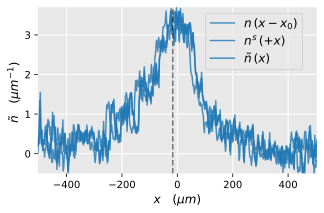
\includegraphics[width=\textwidth]{Figures/article_asymetrie_24-04-2024}
			\caption{(Donnée du 24-04-2024)}
   			\label{fig:asymetrie}	
			\end{subfigure}
			\hfill
    		\begin{subfigure}[b]{0.24\textwidth}
   				 \includegraphics[width=\textwidth]{Figures/article_simul_deformation_1_24-04-2024}
        			\caption{}
        		\label{fig:simul_deformation}
   			\end{subfigure}
    		\hfill
    		\begin{subfigure}[b]{0.24\textwidth}
        		\centering
        		\includegraphics[width=\textwidth]{Figures/article_simul_expansion_1_24-04-2024}
        		\caption{}
        		\label{fig:simul_expansion}
    		\end{subfigure}
    		\hfill
    		\begin{subfigure}[b]{0.24\textwidth}
    			\centering
				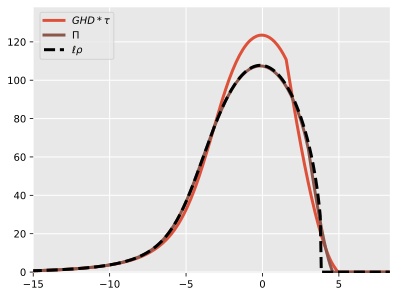
\includegraphics[width=\textwidth]{Figures/article_distribution_24-04-2024}		
				\caption{Donnée du 24-04-2024}
   				\label{}    			
    		\end{subfigure}    		
    		\caption{Donnée du 24-04-2024}
   			\label{}					
		\end{figure}
		
		%Nous commençons par ajuster le profil de déformation du bord en utilisant des simulations GHD  $n_{\mbox{\tiny GHD}}$, en prenant la température $T$ comme paramètre ajustable. Le potentiel chimique $\mu$ est paramétré en fonction de la température et de la densité spatiale initiale du nuage, notée $n_p$.  $\mu$  est ajusté en utilisant un modèle thermique de Yang-Yang afin de retrouver une densité spatiale initiale correspondant à $n_p$, mesurée à $47~(56.6)~\mu \text{m}^{-1}$. L'ajustement optimal de la déformation du bord est obtenu pour une température $T = 966 ~(559)~\text{nK}$ et un potentiel chimique $\mu = 43~(65)~\text{nK}$ (voir courbe orange de la Fig. \ref{fig:simul_deformation}).Sur un intervalle $[-222 , 70] ~([-150 , 100])~\mu \mbox{m}$, $\chi^2 = \Vert (n - n_{\mbox{\tiny GHD}}) / n_{\mbox{\tiny GHD}} \Vert^2_\infty  = ? (?)$ .
		We start by fitting the edge deformation profile using GHD simulations $n_{\mbox{\tiny GHD}}$, with the temperature $T$ as an adjustable parameter. The chemical potential $\mu$ is parameterized as a function of the temperature and the initial spatial density of the cloud, denoted $n_p$. $\mu$ is determined using a Yang-Yang thermal model to match the initial spatial density $n_p$, measured at $47~(56.6)~\mu \text{m}^{-1}$. The optimal fit for the edge deformation is obtained with a temperature $T = 966~(559)~\text{nK}$ and a chemical potential $\mu = 43~(65)~\text{nK}$ (see orange curve in Fig. \ref{fig:simul_deformation}). Over the interval $[-220, 70]~([-150, 100])~\mu \mbox{m}$, $\chi^2 = \Vert (n - n_{\mbox{\tiny GHD}})\Vert^2_\infty  = ? (?) ~ \mu \text{m}^{-2} $.

		
		%Pour déterminer $x_0$, on ajuste les données d'expansion à $\tau = 1~\text{ms}$ avec un modèle de fonction porte convoluée avec une gaussienne, où $x_0$ est le centre de la fonction. J'obtiens $x_0 = 5.7~(18.4)~\mu \text{m}$. Ensuite, on multiplie le profil de bord par une fonction porte centrée en $x_0$ et de diamètre $\ell$. On ajuste $\ell$ pour obtenir, dans la tranche, le même nombre d'atomes que mesuré dans les données à $\tau = 50~(30)~\text{ms}$. On trouve ainsi $\ell = 41.5~(22.2)~\mu \text{m}$ .
		To determine $x_0$, we fit the expansion data at $\tau = 1~\text{ms}$ with a model of a rectangular function convolved with a Gaussian, where $x_0$ is the center of the function. We obtain $x_0 = 5.5~(18.4)~\mu \text{m}$. Next, we multiply the edge profile by a rectangular function centered at $x_0$ with a diameter $\ell$. We adjust $\ell$ to match the number of atoms in the slice to the one measured in the data at $\tau = 50~(30)~\text{ms}$. This gives $\ell = 41.5~(22.2)~\mu \text{m}$.

		
		%Après l'expansion, on observe une asymétrie dans les données, avec un côté plus raide. Cette asymétrie est également visible dans les simulations GHD $\tilde{n}_{\mbox{\tiny GHD}}$ , mais on observe des diference entre les données la les simulations GHD, notament sur la partie de droite non-termique. Sur un intervalle $[-222 , 70] ~([-150 , 100])~\mu \mbox{m}$, $\chi^2 = \Vert (\tilde{n} - \tilde{n}_{\mbox{\tiny GHD}}) / \tilde{n}_{\mbox{\tiny GHD}} \Vert^2_\infty  = ? (?)$ (voir courbe orange de la Fig. \ref{fig:simul_expansion}).  On a envie d'augmenter $T$ et diminuer $x_0$. 
		
		After the expansion, we observe an asymmetry in the data, with one side being steeper. This asymmetry is also visible in the GHD simulations $\tilde{n}_{\mbox{\tiny GHD}}$, but differences are noticeable between the data and the GHD simulations, particularly on the non-thermal right-hand side. Over the interval $[-222 , 70] ~([-150 , 100])~\mu \mbox{m}$, $\chi^2 = \Vert (\tilde{n} - \tilde{n}_{\mbox{\tiny GHD}}) \Vert^2_\infty  = ? (?) ~$ (see orange curve in Fig. \ref{fig:simul_expansion}). We consider increasing $T$ and decreasing $x_0$.

		
		%On a donc fait un ajustement des simulation GHD aus des donnée aprés expansion. On a fait un ajustement avec $T$ et $x_0$ comme parametres ajustables, $\mu$ et $\ell$ gardent les même contraintes que précedement. Les paramètre après cette ajustement sont $T= 1350~(1000) ~ \mbox{nK}$ et $x_0 = -6.7~(17.8)~\mu\mbox{m}$ (voir courbe rouge de la Fig. \ref{fig:simul_expansion}).Sur un intervalle $[-222 , 70] ~([-150 , 100])~\mu \mbox{m}$, $\chi^2 = \Vert (\tilde{n} - \tilde{n}_{\mbox{\tiny GHD}}) / \tilde{n}_{\mbox{\tiny GHD}} \Vert^2_\infty  = ? (?)$ .
		
		We therefore performed a fit of the GHD simulations to the data after expansion. The fit was conducted with $T$ and $x_0$ as adjustable parameters, while $\mu$ and $\ell$ retained the same constraints as previously described. The parameters obtained after this fit are $T = 1350~(1000)~\mbox{nK}$ and $x_0 = -3.18~(17.8)~\mu\mbox{m}$ (see red curve in Fig. \ref{fig:simul_expansion}). Over the interval $[-222, 70]~([-150, 100])~\mu \mbox{m}$, $\chi^2 = \Vert (\tilde{n} - \tilde{n}_{\mbox{\tiny GHD}}) \Vert^2_\infty  = ? (?)~\mu \text{m}^{-2}$.

		
		%Mais maintenant avec c'est nouveau paramêtre les simulation GHD sont moin en accord avec les profils de bords. Sur un intervalle $[-222 , 70] ~([-150 , 100])~\mu \mbox{m}$, $\chi^2 = \Vert (n - n_{\mbox{\tiny GHD}}) / n_{\mbox{\tiny GHD}} \Vert^2_\infty  = ? (?)$ (voir courbe rouge de la Fig. \ref{fig:simul_deformation). {\color{bleu} Et meme les $x_0$ ???}.
		
		However, with these new parameters, the GHD simulations show less agreement with the edge deformation profiles. Over the interval $[-220, 70]~([-150, 100])~\mu \mbox{m}$, $\chi^2 = \Vert (n - n_{\mbox{\tiny GHD}})  \Vert^2_\infty  = ? (?)~ \mu \text{m}^{-2}$ (see red curve in Fig. \ref{fig:simul_deformation}). {\color{blue} And even the $x_0$ ???}.
		

		
		%Hors de l'instervale $[-222 , 70] ~([-150 , 100])~\mu \mbox{m}$ on voit du bruit qui ne sont pas expliqué par les simulation GDH.
		
		Outside the interval $[-222, 70]~([-150, 100])~\mu \mbox{m}$, we observe noise that is not explained by the GHD simulations.

		
		%Les simulation GHD sont déjà pour un temps d'expanstion fini $\tau = 50~(30)~\mbox{ms}$ assez proches au prevision pour $\tau^\ast \to \infty$ , avec $\ell\to 0$ négligeable , la distribution $\rho_{x_0}/\tau*\ell$. La difference notable est un bord verticale non-termique pour $\rho_{x_0}/\tau*\ell$. Pour $\ell$ $\Pi_{x_0 , \ell}/\tau$ ,  non négligeable la difference s'amoindrie. 
		
		The GHD simulations, already performed for a finite expansion time $\tau = 50~(30)~\mbox{ms}$, are quite close to the predictions for $\tau^\ast \to \infty$, with $\ell \to 0$ being negligible, and the distribution $\rho_{x_0}/\tau*\ell$. The notable difference is a non-thermal vertical edge for $\rho_{x_0}/\tau*\ell$. For $\ell$ $\Pi_{x_0 , \ell}/\tau$, as $\ell$ becomes non-negligible, the difference diminishes.
		




 \begin{figure}[!htb]
     \centering
     \includegraphics[width=0.8\linewidth]{Figures/asymetrie_GHD_all.png}
     \caption{A second graph for this last part, change the format (.pdf). Add the profile n(-x) to add. Change the captions with using $\Pi$, the extensive rapidity distribution.}
     \label{fig:local}
 \end{figure}

%%{\color{lightgray}
%%After preparing a semi-infinite homogeneous initial gas, as detailed in subsection (\ref{sub_pisih}), and following an evolution time of $\tau = 18$ ms (as seen in subsection \ref{sub.ed}), we aim to probe the rapidity distribution. 
%%For an initial state whose occupation factor distribution smoothly goes to zero, such as a thermal state, 
%%the occupation factor distribution within the border, is expected    to be highly asymetric according to Eq.\eqref{eq:nuetoile}:  its left side shows a discontinuity similar to that of ground states while its right side shows the smooth behavior of the initial state.  This implies in turn a highly asymetric rapidity local rapidity distribution.  
%%To reveal such a peculiar behavior, we use the protocol described in \cite{dubois_probing_2024} as detailed below. 
%
%%First we let the border expand for a time $t=18$ ms. 
%%{\color{blue}[Il faudra un graphe avec le profil de bord à 18ms pour ces données pour pouvoir visualiser ce que représente 37 $\mu$m.]} To probe the rapidity distribution around $x=0$, we then select the slice of the gas that lies in the interval  $[-\ell/2, \ell/2]$, where $\ell=37~\mu$m. Finally, we let this slice expand in 1D for an expansion time $\tau$  after which we measure the longitudinal density $\tilde{n}(x, {\tau} )$.  
%%The latter reflects the rapidity distribution of the slice $\Pi(\theta)$, %in the limit 
%%$\tau\rightarrow\infty$, is simply the rapidity distribution of the 
%%slice $\Pi(\theta)$: 
%%the asymptotic behavior being  $\lim_{\tau\rightarrow\infty} (\tau \tilde{n}(x, {\tau} )) =\Pi(x/\tau)$. The asymetry of $\Pi$ thus induces an asymetry of  $\tilde{n}(x,\tau)$ in $x$.
%Such an asymetry is seen in the experimental profile obtained for $\tau=50$ ms shown in Fig. (\ref{fig:local}).
%
%{\color{red} Ce qui serait bien: fiter la fonction de bord pour avoir $T$ et $\mu$. Du coup pas besoin de faire de fit ici. Est-ce que le fit de la fonction de bord donne des paramètres proches de ceux obtenus ici ? Si oui, alors faire comme ça. Et du coup reprendre "à l'endroit" la description des différentes approximations.}
%
%{\color{blue} Comme on l'a discuté, reprendre à l'envers. Commencer par le fit avec le modèle "complet". Puis revenir en arrière. Ne pas utiliser $\nu_{YY}$, terminologie non introduite dans ce papier. Faire ref aux eq. 6 et 7 (en disant $c=0$).} To compare it with the expected rapidity density, as explained in section (\ref{sec.GHDpredictions}), we assume that the selection size $\ell$ is negligible (i.e., the gas is homogeneous in the selected region), and that the velocity at $x = 0$ is zero. Under these conditions, {\color{blue} [La phrase qui suit n'a rien à voir avec la taille de la tranche $\ell$.]} GHD theory predicts that during the deformation of the edge, the occupation factor at $x = 0$ follows $\nu^\ast(\theta) = \nu(\theta) \Theta(\theta - \theta^\ast)$, where $\nu$ is the occupation factor of the semi-infinite homogeneous gas, $\Theta$ is the Heaviside function, and $\theta^\ast$ is a rapidity at which the effective velocity is zero ($v^{\text{eff}}_{\nu^\ast}(\theta^\ast) = 0$).{\color{blue} Pas besoin de redire ça, c'est donné Eq. 2-3}
%
%% We seek to determine the occupation factor at $x = 0$ during the edge spreading. To follow the edge dynamics, we use GHD theory. Initially, we assume that the selection size is zero ($\ell = 0$), which is equivalent to assuming that the gas is homogeneous within the selected slice. Under these conditions, let $\theta^\ast$ be a rapidity, and we denote $\nu_{\theta^\ast}$ as the occupation factor defined by:
%% \begin{eqnarray}
%% 	\nu_{\theta^\ast} & = & \left \{ \begin{array}{rcl} 0 & \mbox{if} & \theta > \theta^\ast, \\ \nu (\theta ) & \mbox{otherwise} & \end{array} \right .
%% \end{eqnarray} 
%% During the evolution, the occupation factor is $\nu_{\theta^\ast}$, where $\theta^\ast$ is such that the effective velocity $v^{\mbox{eff}}_{\nu_{\theta^\ast}}(\theta^\ast) = 0$.
%
%We fit the occupation factor $\nu$ using a Yang-Yang distribution, $\nu_{YY}(\theta ; \mu_{YY}, T_{YY})$, where $\mu_{YY}$ is the chemical potential and $T_{YY}$ is the temperature of the initial gas, based on GHD simulations of the edge deformation {\color{blue} [pas assez précis. Et l'expansion ?]}. The fitting parameters are $\mu_{YY} = ??$ nK and $T_{YY} = ??$ nK. After 18 ms of deformation, the rapidity distribution at $x = 0$, denoted $\rho_{\ell \to 0}$, is represented by the green curve in Fig. (\ref{fig:local}). This distribution is also asymmetric and shares similarities with experimental results, although with a noticeable difference: it shows a sharp left edge, a hallmark of a non-thermal boundary (see \cite{lieb_exact_1963}).
%
%When accounting for the finite selection size $\ell$, the rapidity distribution edge, $\Pi_{\ell = 37 \mu m}$, exhibits both a rough and a smoother region, as illustrated by the solid black curve in Fig. (\ref{fig
%}), which is more consistent with experimental data. Comparing these curves suggests that with a longer 1D expansion time $\tilde{\tau}$, the left edge of the profile would steepen and the profiles would approach the rapidity distribution $\Pi_{\ell = 37 \mu m}$. Ultimately, rapidity distributions are attained for an infinite expansion time. As GHD theory accurately describes 1D expansion dynamics, we use it to predict the system's behavior. A GHD simulation for $\tilde{\tau} = 50$ ms is represented by the dotted black curve in Fig. (\ref{fig:local}).
%
%
%
%{\color{magenta}
% \begin{itemize}
%     \item GHD simulations predict locally a non thermal and asymetric rapidity distribution at the edge deformation. Maybe we can explain technical things about the simulations
%     \item Describe the experimental protocol, referring to the previous article.  
%     \item Experimental data, profile asymmetry highlighted
%     \item First comparison with the assumed homogeneous rapidity distribution in the slice
%     \item Second comparison with the inhomogeneous rapidity distribution in the slice
%     \item Third comparison with the GHD simulations to take into account the fact that the asymptotic regime is not completely reached.
% \end{itemize}
% }
% }

\section{Conclusion}
\begin{itemize}
    \item a protocol that could enable the study of zero-entropy physics
\end{itemize}

\section*{Acknowledgements}

% \paragraph{Author contributions}
% This is optional. If desired, contributions should be succinctly described in a single short paragraph, using author initials.

\paragraph{Funding information}





\begin{appendix}


\section{Details of calculations}
%\subsection{Usefull formulas }
Let us first introduce notations and usefull formulas. 
In the context of this paper, for an occupation factor distribution $\nu_0(\theta)$, we define the dressing  as
\begin{equation}
	\label{eq:dressing}
f^{\rm dr}(\theta^*,\theta) = f(\theta) + \int_{-\infty}^{\theta^*}\frac{d\theta'}{2\pi}   \Delta(\theta-\theta') \nu_0 (\theta') f^{\rm dr}(\theta^*,\theta') .
\end{equation}
The two following formulas are useful for our purposes:
\begin{itemize}
	\item variation of a dressed quantity at `Riemann point'
		 \begin{equation}
		 	\label{eq:variation_fdr_Rp}
     \frac{d   f^{\rm dr}(\theta^*,\theta^* ) }{d\theta^*} = -  \nu_0 (\theta^*) f^{\rm dr}(\theta^*,\theta^*)  \, \frac{[ \Delta(.-\theta^*) ]^{\rm dr}(\theta^*,\theta ^*)}{2\pi} +  f' (\theta^*)  +  \int_{-\infty}^{\theta^*}  \Delta'(\theta^*-\theta')  \nu_0 (\theta') f^{\rm dr}(\theta^*,\theta')  \frac{d\theta'}{2\pi}  ,       
	%\delta (  f^{\rm dr}(\theta^* ) ) = \left(  -  \nu (\theta^*) f^{\rm dr}(\theta^*)  \, \frac{[ \varphi(.-\theta^*) ]^{\rm dr}(\theta^*)}{2\pi} +  f' (\theta^*)  +  \int^\infty_{\theta^*}  \varphi'(\theta^*-\theta')  \nu (\theta') f^{\rm dr}(\theta')  \frac{d\theta'}{2\pi}  \right) \delta \theta^*,
	\end{equation}
%		 \begin{equation}
%		 	\label{eq:variation_fdr_Rp}
%	\delta (  f^{\rm dr}(\theta^* ) ) = \left(  (f')^{\rm dr} (\theta^*)  +  \int^\infty_{\theta^*}  [\varphi(.-\theta')]^{\rm dr}(\theta^*)  \nu' (\theta') f^{\rm dr}(\theta')  \frac{d\theta'}{2\pi}  \right) \delta \theta^*,
%	\end{equation}
	\item variation of a charge density
		 \begin{equation}
		 	\label{eq:variation_Q}
            \frac{d \left ( \int_{\theta^*}^\infty \frac{d \theta}{2\pi} \nu_0 (\theta)   f^{\rm dr}(\theta^*,\theta)\right )}{d\theta^*}=
            - \nu_0(\theta^*) \frac{1^{\rm dr} (\theta^*,\theta^*)  f^{\rm dr} (\theta^*,\theta^*)}{2\pi} 
			%\delta \left(  \int_{\theta^*}^\infty \frac{d \theta}{2\pi} \nu (\theta)   f^{\rm dr}(\theta) \right)  =    - \nu(\theta^*) \frac{1^{\rm dr} (\theta^*)  f^{\rm dr} (\theta^*)}{2\pi}  \delta \theta^* .
		\end{equation}	
\end{itemize}


These formulas can be derived as follows. Varying the definition of the dressing (\ref{eq:dressing}) w.r.t $\theta^*$, we get
\begin{equation*}
	\label{eq:var1}
\frac{d ( f^{\rm dr}(\theta^*,\theta) )}{d\theta^*}  =  -  \nu_0 (\theta^*) f^{\rm dr}(\theta^*,\theta^*) \, \frac{[ \Delta(.-\theta^*) ]^{\rm dr}(\theta^*,\theta)}{2\pi} .
\end{equation*}
Eq.~\eqref{eq:variation_fdr_Rp} follows. 
Then the variation of the charge density is
\begin{eqnarray*}
\nonumber			\frac{d \left(  \int^{\theta^*}_{-\infty} \frac{d \theta}{2\pi} \nu_0 (\theta)   f^{\rm dr}(\theta^*,\theta) \right)}{d\theta^*}  \nonumber &=&  -\frac{1}{2\pi} \nu_0(\theta^*) f^{\rm dr} (\theta^*,\theta^*)    - \nu_0 (\theta^*) f^{\rm dr}(\theta^*,\theta^*) \int_{\theta^*}^\infty \frac{d\theta   }{2\pi}  \nu_0 (\theta)   \frac{[ \Delta(.-\theta^*) ]^{\rm dr}(\theta^*,\theta)}{2\pi}   .\\
%\nonumber &=& -\frac{1}{2\pi} \nu(\theta^*) f^{\rm dr} (\theta^*)  \delta \theta^*  \left[  1+ \int_{\theta^*}^\infty \frac{d\theta   }{2\pi} 1^{\rm dr}(\theta) \nu (\theta)   \varphi(\theta-\theta^*) \right] \\
%\nonumber &=& - \nu(\theta^*) f^{\rm dr} (\theta^*) \frac{1^{\rm dr} (\theta^*)}{2\pi}  \delta \theta^* ,
%\nonumber			\delta \left(  \int_{\theta^*}^\infty \frac{d \theta}{2\pi} \nu (\theta)   f^{\rm dr}(\theta) \right)  \nonumber &=&  -\frac{1}{2\pi} \nu(\theta^*) f^{\rm dr} (\theta^*)  \delta \theta^*  - \nu (\theta^*) f^{\rm dr}(\theta^*) \delta \theta^*  \int_{\theta^*}^\infty \frac{d\theta   }{2\pi}  \nu (\theta)   \frac{[ \varphi(.-\theta^*) ]^{\rm dr}(\theta)}{2\pi}   \\
%\nonumber &=& -\frac{1}{2\pi} \nu(\theta^*) f^{\rm dr} (\theta^*)  \delta \theta^*  \left[  1+ \int_{\theta^*}^\infty \frac{d\theta   }{2\pi} 1^{\rm dr}(\theta) \nu (\theta)   \varphi(\theta-\theta^*) \right] \\
%\nonumber &=& - \nu(\theta^*) f^{\rm dr} (\theta^*) \frac{1^{\rm dr} (\theta^*)}{2\pi}  \delta \theta^* ,
\end{eqnarray*}	
One then uses the fact that, for any functions $g$ and $h$,  $\int d\theta\nu(\theta)h^{\rm dr} g = 
\int d\theta\nu(\theta)h g^{\rm dr} $ to transform the integral in the r.h.s into $\int d\theta/(2\pi)\Delta(\theta-\theta^*)1^{\rm dr}(\theta^*,\theta)$. 
One then obtain formula (\ref{eq:variation_Q}). %Differentiating the definition of the dressing (\ref{eq:dressing}) w.r.t $\theta$ and using Eq. (\ref{eq:var1}) we arrive at formula (\ref{eq:variation_fdr_Rp}).

%\subsection{Deriving Eq.}
Let us now derive Eq.~\eqref{eq:dndtheta}. For simplicity let us denote $v^{\rm eff}(\theta^*)$
the quantity $ v^{\rm eff}_{\nu^*}(\theta^*)$ where 
$\nu^*$ is defined Eq.\ref{eq:nuetoile}.
Let us introduce $A(\theta^*)=dv^{\rm eff}/d\theta^*$. Using $v^{\rm eff} = \theta^{\rm dr}/1^{\rm dr}$ and using above formulas one finds
\begin{eqnarray}
%\nonumber   A [\nu] (\theta^*)  &  \overset{{\rm def}}{=} & 	\frac{\delta ( v^{\rm eff}(\theta^*) )}{\delta %\theta^*} \\
%&=& \frac{1}{1^{\rm dr} (\theta^*)}  \left( 1 + \int_{\theta^*}^\infty \varphi'(\theta^* - \theta) [ {\rm id}^{\rm dr}(\theta) - v^{\rm eff}(\theta^*) 1^{\rm dr}(\theta)  ]  \nu(\theta) \frac{d\theta}{2\pi} \right) 
\nonumber   A (\theta^*)  &=& \frac{1}{1^{\rm dr} (\theta^*,\theta^*)}  \left( 1 + \int^{\theta^*}_{-\infty} \Delta'(\theta^* - \theta) [ {\rm id}^{\rm dr}(\theta^*,\theta) - v^{\rm eff}(\theta^*) 1^{\rm dr}(\theta^*,\theta)  ]  \nu_0(\theta) \frac{d\theta}{2\pi} \right) .
\end{eqnarray}
Let us now introduce $B(\theta^*)$ as $= %$ as %and $D [\nu] = A[\nu] / B[\nu]$ with
%\begin{eqnarray}
%  \nonumber   B[\nu] (\theta^*) \, \nu (\theta^*) &  \overset{{\rm def}}{=} & 
%\frac{ \delta ( n(\theta^*) ) }{\delta \theta^*} \\
% &=& - \frac{1^{\rm dr} (\theta^*)^2}{2\pi}    \, \nu (\theta^*)   \, .
%\end{eqnarray}
%\begin{eqnarray}
  %\nonumber   
  B(\theta^*) \, \nu_0 (\theta^*) %&  \overset{{\rm def}}{=} & 
  =
{ d ( n(\theta^*) ) }/{d \theta^*} $
%$,\\
%\end{eqnarray}
where $n(\theta^*)=\int_{-\infty}^{\theta^*} d\theta \nu_0(\theta)1^{\rm dr}(\theta^*,\theta)$ is the linear density for the occupation factor distribution $\nu^*$.
Using above formulas we obtain
\begin{eqnarray}
  \nonumber   B(\theta^*)  &=& - \frac{1^{\rm dr} (\theta^*,\theta^*)^2}{2\pi}      \, .
\end{eqnarray}
%Let us now introduce $D (\theta^*) = A(\theta^*) / B(\theta^*)$.  
{\color{blue} A discuter. $A$ and $B$ are functionals of $\nu_0$ whose functional derivatives $\frac{\delta A}{\delta \nu (\theta)}$, $\frac{\delta B}{\delta \nu (\theta)}$, $\frac{\delta D}{\delta \nu (\theta)}$ are smooth at $\theta = \theta^*$.}
%Let us define $D [\nu] = A[\nu] / B[\nu]$ so that
Let us now consider the border function $n(v)$ and the edge rapidity $\theta^*(v)$, defined in eq.\ref{}. Using $dn/dv=(dn/d\theta^*)(d\theta^*/d v)$ and the fact that $v=v^{\rm eff}(\theta^*)$, one finds 
\begin{equation}
	\nu (\theta^*) \, = \, \frac{A(\theta^*)}{B(\theta^*)} \frac{dn}{dv} .
\end{equation}
Introducing 
$D=A/B$ and differentiating w.r.t $\theta^*$  this gives Eq.~(\ref{eq:dndtheta}).


\end{appendix}


% \section{First appendix}
% Add material which is better left outside the main text in a series of Appendices labeled by capital letters.

% \section{About references}
% Your references should start with the comma-separated author list (initials + last name), the publication title in italics, the journal reference with volume in bold, start page number, publication year in parenthesis, completed by the DOI link (linking must be implemented before publication). If using BiBTeX, please use the style files provided  on \url{https://scipost.org/submissions/author_guidelines}. If you are using our \LaTeX template, simply add
% \begin{verbatim}
% \bibliography{your_bibtex_file}
% \end{verbatim}
% at the end of your document. If you are not using our \LaTeX template, please still use our bibstyle as
% \begin{verbatim}
% \bibliographystyle{SciPost_bibstyle}
% \end{verbatim}
% in order to simplify the production of your paper.
% \end{appendix}


% TODO:
% Provide your bibliography here. You have two options:

% FIRST OPTION - write your entries here directly, following the example below, including Author(s), Title, Journal Ref. with year in parentheses at the end, followed by the DOI number.
%\begin{thebibliography}{99}
%\bibitem{1931_Bethe_ZP_71} H. A. Bethe, {\it Zur Theorie der Metalle. i. Eigenwerte und Eigenfunktionen der linearen Atomkette}, Zeit. f{\"u}r Phys. {\bf 71}, 205 (1931), \doi{10.1007\%2FBF01341708}.
%\bibitem{arXiv:1108.2700} P. Ginsparg, {\it It was twenty years ago today... }, \url{http://arxiv.org/abs/1108.2700}.
%\end{thebibliography}

% SECOND OPTION:
% Use your bibtex library
% \bibliographystyle{SciPost_bibstyle}
\bibliography{Biblio_Lea.bib,Domain_Wall_paper}

\nolinenumbers

\end{document}
